%%%%%%%%%%%%%%%%%%%%%%%%%%%%%%%%%%%%
%% PREAMBLE
%%%%%%%%%%%%%%%%%%%%%%%%%%%%%%%%%%%%

\documentclass[11pt]{article}

% packages needed for state diagrams
\usepackage{pgf}
\usepackage{tikz}
\usetikzlibrary{arrows,automata}

% page margins
\usepackage[margin=2.5cm]{geometry}
\setlength{\parindent}{0pt}

\begin{document}

\begin{center}
    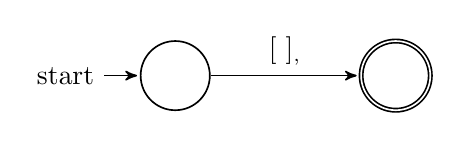
\begin{tikzpicture}[->,>=stealth',shorten >=1pt,auto,node distance=2.8cm,semithick]
        \tikzstyle{every state}=[fill=white,draw=black,text=black]
        \node[initial,state] (s0) {};
        \node[state,accepting] (s1) [right of=s0] {};
    \path
        (s0) edge node {$[\ ]_{,}$} (s1);
    \end{tikzpicture}
\end{center}

\bigskip

\begin{center}
    \begin{tikzpicture}[->,>=stealth',shorten >=1pt,auto,node distance=2.8cm,semithick]
        \tikzstyle{every state}=[fill=white,draw=black,text=black]
        \node[initial,state] (s0) {};
        \node[state] (s1) [right of=s0] {};
        \node[state] (s2) [below of=s1] {};
        \node[state] (s3) [below of=s2] {};
        \node[state,accepting,rectangle] (s4) [right of=s1] {$[\ ]_{,}$};
    \path
        (s0) edge node {[} (s1)
        (s1) edge node {]} (s4) edge node {$[\ ]_{,}$} (s2)
        (s2) edge [bend right] node [swap] {'} (s3) edge [bend right] node {]} (s4)
        (s3) edge [bend right] node [swap] {$[\ ]_{,}$} (s2);
    \end{tikzpicture}
\end{center}
\end{document}
